\documentclass[11pt]{article}

\usepackage[margin=1in]{geometry}
\usepackage{amsmath, amssymb, amsthm}
\usepackage{tikz}
\usetikzlibrary{arrows.meta, decorations.pathreplacing, angles, quotes, calc}
\usepackage{hyperref}
\usepackage{microtype}
\usepackage{parskip}

\newtheorem{theorem}{Theorem}
\newtheorem{proposition}[theorem]{Proposition}

\newcommand{\vect}[1]{\mathbf{#1}}
\newcommand{\ihat}{\hat{\imath}}
\newcommand{\jhat}{\hat{\jmath}}
\newcommand{\khat}{\hat{k}}
\newcommand{\norm}[1]{\left\lVert #1 \right\rVert}

\title{A Deep Dive into the Dot Product}
\author{Dave Rosenman \\ \texttt{dave.rosenman.data@gmail.com}}
\date{April 19, 2026}

\begin{document}
\maketitle

\section{Two Definitions}

The dot product of two vectors $\vect{a}$ and $\vect{b}$ in $\mathbb{R}^3$ is usually introduced in one of two seemingly unrelated ways.

\textbf{Algebraic definition.} If $\vect{a} = \langle a_x, a_y, a_z \rangle$ and $\vect{b} = \langle b_x, b_y, b_z \rangle$, then
\[
  \vect{a} \cdot \vect{b} \;=\; a_x b_x + a_y b_y + a_z b_z.
\]

\textbf{Geometric definition.} If $\theta$ is the angle between $\vect{a}$ and $\vect{b}$, then
\[
  \vect{a} \cdot \vect{b} \;=\; \norm{\vect{a}}\,\norm{\vect{b}}\,\cos\theta.
\]

The first is a rule for combining six numbers. The second is a statement about geometry that never mentions a coordinate system at all. How can they describe the same object?

The goal of this article is to:
\begin{enumerate}
  \item Build the geometric intuition behind $\norm{\vect{a}}\norm{\vect{b}}\cos\theta$ — it is really measuring a \emph{projection}.
  \item Prove that the two definitions are equivalent.
  \item Use the geometric definition to show that the dot product is \emph{coordinate-system invariant}: even though the six numbers $a_x,\dots,b_z$ all change when you rotate your axes, the sum $a_x b_x + a_y b_y + a_z b_z$ never does.
  \item Prove that perpendicular vectors have dot product zero — twice. Once from $\cos 90^\circ = 0$, and once by using invariance to rotate the vectors onto the axes and read off that the component formula gives zero.
\end{enumerate}

\section{The Geometric Picture: Projection}

The geometric definition $\vect{a}\cdot\vect{b} = \norm{\vect{a}}\norm{\vect{b}}\cos\theta$ looks arbitrary until you see that it is measuring \emph{projection}.

Drop a perpendicular from the tip of $\vect{a}$ onto the line through $\vect{b}$. The length of the shadow that $\vect{a}$ casts onto that line is
\[
  \norm{\vect{a}}\cos\theta,
\]
called the \emph{scalar projection} of $\vect{a}$ onto $\vect{b}$. Intuitively, it measures ``how much of $\vect{a}$ points along $\vect{b}$.''

\begin{center}
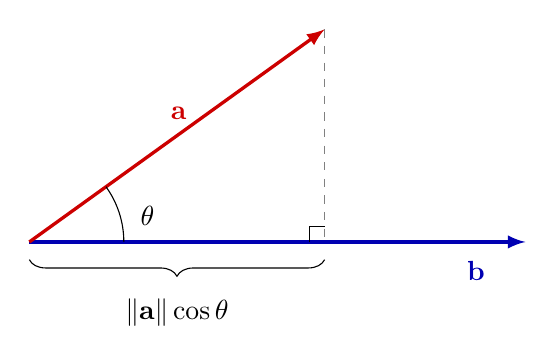
\begin{tikzpicture}[scale=1.5, >=latex]
  \coordinate (O) at (0,0);
  \coordinate (A) at (2.5, 1.8);
  \coordinate (B) at (4.2, 0);
  \coordinate (P) at (2.5, 0);

  \draw[->, very thick, blue!70!black] (O) -- (B) node[pos=0.9, below=3pt] {$\vect{b}$};
  \draw[->, very thick, red!80!black] (O) -- (A) node[pos=0.55, above left=-2pt] {$\vect{a}$};
  \draw[dashed, gray] (A) -- (P);
  % right angle marker at P
  \draw (P) ++(-0.13,0) -- ++(0,0.13) -- ++(0.13,0);
  % angle arc
  \draw (0.8,0) arc[start angle=0, end angle=35.75, radius=0.8];
  \node at (1.0, 0.22) {$\theta$};
  % brace for projection length
  \draw[decorate, decoration={brace, mirror, amplitude=6pt}] (0,-0.15) -- (2.5,-0.15);
  \node at (1.25, -0.6) {$\norm{\vect{a}}\cos\theta$};
\end{tikzpicture}
\end{center}

\subsection*{Why the shadow has length $\norm{\vect{a}}\cos\theta$ --- from the Pythagorean theorem}

This one spot is where the Pythagorean theorem is doing quiet but essential work, so it is worth spelling out explicitly.

Isolate the right triangle formed in the figure above: the hypotenuse is $\vect{a}$ itself (length $\norm{\vect{a}}$), the side along the $\vect{b}$-line has some length $s$ (the shadow we are trying to measure), and the dashed perpendicular drop has some length $h$.

\begin{center}
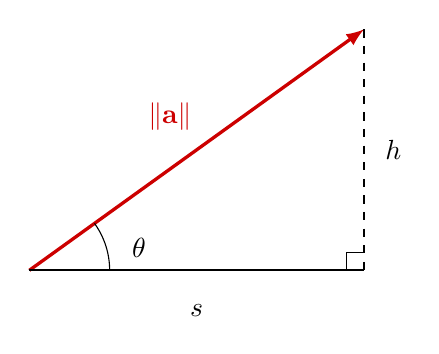
\begin{tikzpicture}[scale=1.7, >=latex]
  \coordinate (O) at (0,0);
  \coordinate (A) at (2.5, 1.8);
  \coordinate (P) at (2.5, 0);

  % the triangle
  \draw[->, very thick, red!80!black] (O) -- (A);
  \node[red!80!black] at (1.05, 1.15) {$\norm{\vect{a}}$};
  \draw[dashed, thick] (A) -- (P);
  \node at (2.72, 0.9) {$h$};
  \draw[thick] (O) -- (P);
  \node at (1.25, -0.3) {$s$};
  % right angle marker at P
  \draw (P) ++(-0.13,0) -- ++(0,0.13) -- ++(0.13,0);
  % angle theta at origin
  \draw (0.6,0) arc[start angle=0, end angle=35.75, radius=0.6];
  \node at (0.82, 0.17) {$\theta$};
\end{tikzpicture}
\end{center}

The Pythagorean theorem relates the three sides:
\[
  s^2 + h^2 \;=\; \norm{\vect{a}}^2.
\]
Divide through by $\norm{\vect{a}}^2$:
\[
  \left(\frac{s}{\norm{\vect{a}}}\right)^2 + \left(\frac{h}{\norm{\vect{a}}}\right)^2 \;=\; 1.
\]
This is the equation of the unit circle. The point
\(\bigl(s/\norm{\vect{a}},\; h/\norm{\vect{a}}\bigr)\)
lies on a circle of radius $1$ --- and it is the point at angle $\theta$ on that circle, because $\theta$ is exactly the angle the hypotenuse $\vect{a}$ makes with its adjacent side. By the unit-circle definition of the trigonometric functions, the point at angle $\theta$ on the unit circle has coordinates $(\cos\theta,\,\sin\theta)$, so
\[
  \frac{s}{\norm{\vect{a}}} \;=\; \cos\theta, \qquad \frac{h}{\norm{\vect{a}}} \;=\; \sin\theta.
\]
Multiplying back by $\norm{\vect{a}}$:
\[
  \boxed{\,s \;=\; \norm{\vect{a}}\cos\theta, \qquad h \;=\; \norm{\vect{a}}\sin\theta.\,}
\]
The shadow on the $\vect{b}$-line has length $\norm{\vect{a}}\cos\theta$, and the perpendicular drop has length $\norm{\vect{a}}\sin\theta$ --- both popping out of the same application of Pythagoras.

\subsection*{Back to the dot product}

The dot product is then this projection times the length of $\vect{b}$:
\[
  \vect{a}\cdot\vect{b} \;=\; \underbrace{\norm{\vect{a}}\cos\theta}_{\substack{\text{how much of }\vect{a}\\ \text{lies along }\vect{b}}} \;\times\; \underbrace{\norm{\vect{b}}}_{\text{length of }\vect{b}}.
\]

By symmetry — and you can verify this from the figure by instead dropping a perpendicular from the tip of $\vect{b}$ onto $\vect{a}$ — it is also $\norm{\vect{b}}\cos\theta$ times $\norm{\vect{a}}$. Either reading gives the same number.

This is why the dot product shows up all over physics: ``work equals force dot displacement'' is really ``force in the direction of motion, times distance traveled.'' Only the component of the force along the path does any work; the perpendicular component is wasted. The dot product isolates exactly the component that matters.

\section{Three Algebraic Properties, from the Geometry Alone}

Before proving the two formulas agree, we derive three algebraic properties using only the geometric definition. These properties are what let us translate between the coordinate-free and the component pictures.

\subsection*{Symmetry}

The angle $\theta$ between $\vect{a}$ and $\vect{b}$ is the same angle between $\vect{b}$ and $\vect{a}$, so
\[
  \vect{a}\cdot\vect{b} = \norm{\vect{a}}\norm{\vect{b}}\cos\theta = \norm{\vect{b}}\norm{\vect{a}}\cos\theta = \vect{b}\cdot\vect{a}.
\]

\subsection*{Scalar multiplication}

For any scalar $c$,
\[
  (c\vect{a})\cdot\vect{b} \;=\; c\,(\vect{a}\cdot\vect{b}).
\]

If $c>0$, scaling $\vect{a}$ by $c$ multiplies its length by $c$ and leaves the angle unchanged, so the dot product scales by $c$. If $c<0$, the length is multiplied by $|c|$ but the vector is flipped, so the new angle is $\pi-\theta$, and $\cos(\pi-\theta) = -\cos\theta$. The two sign changes combine: $|c|\cdot(-\cos\theta) = c\cos\theta$. If $c=0$ both sides are zero.

\subsection*{Distributivity (the interesting one)}

\[
  (\vect{u}+\vect{v})\cdot\vect{w} \;=\; \vect{u}\cdot\vect{w} + \vect{v}\cdot\vect{w}.
\]

Divide both sides by $\norm{\vect{w}}$. The equation becomes
\[
  \text{proj}_{\vect{w}}(\vect{u}+\vect{v}) \;=\; \text{proj}_{\vect{w}}(\vect{u}) + \text{proj}_{\vect{w}}(\vect{v}),
\]
where $\text{proj}_{\vect{w}}(\vect{x}) = \norm{\vect{x}}\cos(\text{angle between }\vect{x},\vect{w})$ is the scalar projection of $\vect{x}$ onto the line through $\vect{w}$.

This is just the statement that \emph{shadows add up}. Place $\vect{v}$ head-to-tail on $\vect{u}$. Then $\vect{u}+\vect{v}$ is the arrow from the tail of $\vect{u}$ to the head of $\vect{v}$. When you drop perpendiculars onto the $\vect{w}$-line, the shadow of $\vect{u}+\vect{v}$ is exactly the shadow of $\vect{u}$ followed by the shadow of $\vect{v}$:

\begin{center}
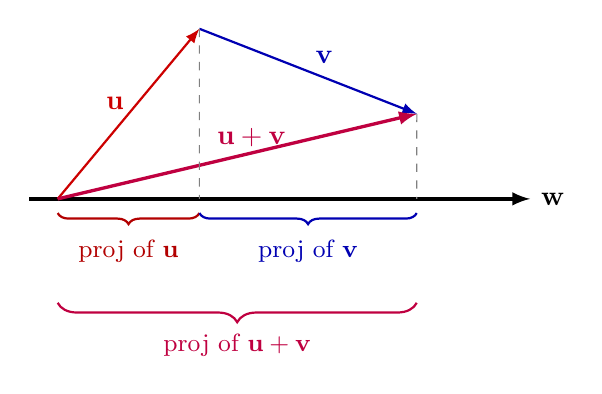
\begin{tikzpicture}[scale=1.2, >=latex]
  \coordinate (O) at (0,0);
  \coordinate (U) at (1.5, 1.8);
  \coordinate (UV) at (3.8, 0.9);

  \draw[->, very thick] (-0.3, 0) -- (5, 0) node[right] {$\vect{w}$};
  \draw[->, thick, red!80!black] (O) -- (U) node[midway, above left=-2pt] {$\vect{u}$};
  \draw[->, thick, blue!70!black] (U) -- (UV) node[midway, above right=-1pt] {$\vect{v}$};
  \draw[->, very thick, purple] (O) -- (UV);
  \node[purple] at (2.05, 0.65) {$\vect{u}+\vect{v}$};

  \draw[dashed, gray] (U) -- (1.5, 0);
  \draw[dashed, gray] (UV) -- (3.8, 0);

  \draw[decorate, decoration={brace, mirror, amplitude=4pt}, red!70!black, thick]
    (0,-0.15) -- (1.5,-0.15);
  \node[red!70!black] at (0.75, -0.55) {\small proj of $\vect{u}$};
  \draw[decorate, decoration={brace, mirror, amplitude=4pt}, blue!70!black, thick]
    (1.5,-0.15) -- (3.8,-0.15);
  \node[blue!70!black] at (2.65, -0.55) {\small proj of $\vect{v}$};
  \draw[decorate, decoration={brace, mirror, amplitude=7pt}, purple, thick]
    (0,-1.1) -- (3.8,-1.1);
  \node[purple] at (1.9, -1.55) {\small proj of $\vect{u}+\vect{v}$};
\end{tikzpicture}
\end{center}

The red segment plus the blue segment exactly equals the purple segment. That is the entirety of the argument. Multiplying back by $\norm{\vect{w}}$ recovers the distributive law for the dot product.

By symmetry, the dot product is also distributive in its first slot: $\vect{u}\cdot(\vect{v}+\vect{w}) = \vect{u}\cdot\vect{v} + \vect{u}\cdot\vect{w}$.

\section{Proving the Two Definitions Agree}

Armed with linearity, the equivalence is a short calculation.

\begin{theorem}
Let $\vect{a} = a_x\ihat + a_y\jhat + a_z\khat$ and $\vect{b} = b_x\ihat + b_y\jhat + b_z\khat$, where $\ihat,\jhat,\khat$ are the standard orthonormal unit vectors along the $x$-, $y$-, and $z$-axes. Then
\[
  \norm{\vect{a}}\,\norm{\vect{b}}\,\cos\theta \;=\; a_x b_x + a_y b_y + a_z b_z.
\]
\end{theorem}

\begin{proof}
First evaluate the dot product of each basis vector with itself and with the others using the geometric definition. Each $\ihat,\jhat,\khat$ has length $1$. The angle between any two distinct ones is $90^\circ$, and the angle between one and itself is $0^\circ$:
\[
  \ihat\cdot\ihat = 1\cdot 1\cdot\cos 0 = 1,
  \qquad
  \ihat\cdot\jhat = 1\cdot 1\cdot\cos\tfrac{\pi}{2} = 0,
\]
and similarly
\[
  \jhat\cdot\jhat = \khat\cdot\khat = 1,
  \qquad
  \ihat\cdot\khat = \jhat\cdot\khat = 0.
\]

Now expand $\vect{a}\cdot\vect{b}$ using the distributivity and scalar properties from the previous section:
\begin{align*}
  \vect{a}\cdot\vect{b}
  &= (a_x\ihat + a_y\jhat + a_z\khat)\cdot(b_x\ihat + b_y\jhat + b_z\khat) \\[2pt]
  &= a_x b_x (\ihat\cdot\ihat) + a_x b_y (\ihat\cdot\jhat) + a_x b_z (\ihat\cdot\khat) \\
  &\quad + a_y b_x (\jhat\cdot\ihat) + a_y b_y (\jhat\cdot\jhat) + a_y b_z (\jhat\cdot\khat) \\
  &\quad + a_z b_x (\khat\cdot\ihat) + a_z b_y (\khat\cdot\jhat) + a_z b_z (\khat\cdot\khat) \\[2pt]
  &= a_x b_x\cdot 1 + a_y b_y\cdot 1 + a_z b_z\cdot 1 \;+\; (\text{six zeros}) \\[2pt]
  &= a_x b_x + a_y b_y + a_z b_z. \qedhere
\end{align*}
\end{proof}

That is the whole story. The algebraic formula is not an independent definition — it is what the geometric definition becomes when you expand the vectors in an orthonormal basis and use the relations $\ihat\cdot\ihat=1$ and $\ihat\cdot\jhat=0$. The six cross-terms like $a_x b_y(\ihat\cdot\jhat)$ vanish \emph{because} $\ihat$ and $\jhat$ are perpendicular, and the three surviving terms are each ``the shadow of $\vect{a}$ on an axis, times the shadow of $\vect{b}$ on the same axis.''

\section{Coordinate-System Invariance}

The geometric definition
\[
  \vect{a}\cdot\vect{b} = \norm{\vect{a}}\,\norm{\vect{b}}\cos\theta
\]
refers to three quantities: two lengths and one angle. None of them depend on a coordinate system.

The length $\norm{\vect{a}}$ is a physical number — how long the arrow is. Rotating the axes does not move the arrow, so its length is unchanged. Likewise for $\norm{\vect{b}}$. The angle $\theta$ is the physical angle between the two arrows; it has nothing to do with which direction you happen to be calling the $x$-axis.

\begin{proposition}
The dot product $\vect{a}\cdot\vect{b}$ is invariant under rotation of the coordinate system.
\end{proposition}

This is a striking fact, because the six numbers $a_x, a_y, a_z, b_x, b_y, b_z$ are \emph{not} invariant — rotate your axes and every one of them changes. Yet the specific combination
\[
  a_x b_x + a_y b_y + a_z b_z \;=\; a_{x'} b_{x'} + a_{y'} b_{y'} + a_{z'} b_{z'}
\]
holds for \emph{any} choice of rotated orthonormal axes $x',y',z'$. The sum conspires to stay fixed even though the individual terms shift around.

\begin{center}
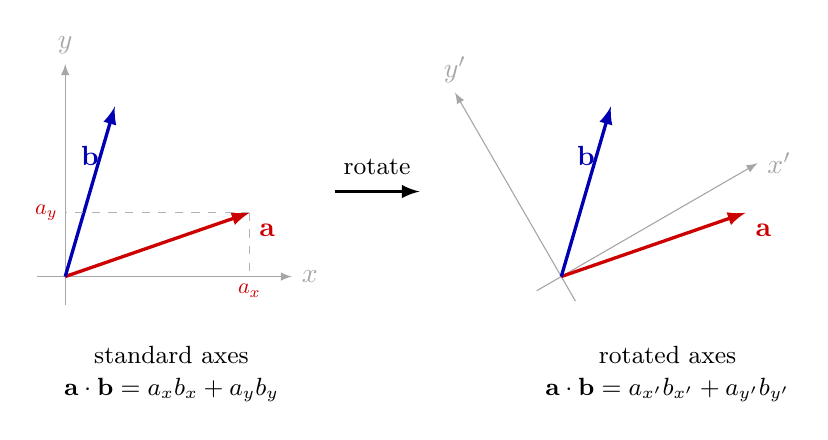
\begin{tikzpicture}[>=latex, scale=0.9]
  % Scene A: standard axes
  \begin{scope}
    \draw[->, thin, gray!70] (-0.4, 0) -- (3.2, 0) node[right] {$x$};
    \draw[->, thin, gray!70] (0, -0.4) -- (0, 3) node[above] {$y$};
    \draw[->, very thick, red!80!black] (0,0) -- (2.6, 0.9);
    \node[red!80!black] at (2.85, 0.65) {$\vect{a}$};
    \draw[->, very thick, blue!70!black] (0,0) -- (0.7, 2.4);
    \node[blue!70!black] at (0.35, 1.7) {$\vect{b}$};
    \draw[dashed, gray!60] (2.6, 0.9) -- (2.6, 0) node[below, red!80!black, scale=0.8] {$a_x$};
    \draw[dashed, gray!60] (2.6, 0.9) -- (0, 0.9) node[left, red!80!black, scale=0.8] {$a_y$};
    \node at (1.5, -1.1) {\small standard axes};
    \node at (1.5, -1.6) {\small $\vect{a}\cdot\vect{b} = a_x b_x + a_y b_y$};
  \end{scope}
  % Arrow
  \draw[->, very thick] (3.8, 1.2) -- (5, 1.2);
  \node at (4.4, 1.55) {\small rotate};
  % Scene B: rotated axes, same vectors
  \begin{scope}[xshift=7cm]
    \draw[->, thin, gray!70, rotate around={30:(0,0)}] (-0.4, 0) -- (3.2, 0) node[right] {$x'$};
    \draw[->, thin, gray!70, rotate around={30:(0,0)}] (0, -0.4) -- (0, 3) node[above] {$y'$};
    \draw[->, very thick, red!80!black] (0,0) -- (2.6, 0.9);
    \node[red!80!black] at (2.85, 0.65) {$\vect{a}$};
    \draw[->, very thick, blue!70!black] (0,0) -- (0.7, 2.4);
    \node[blue!70!black] at (0.35, 1.7) {$\vect{b}$};
    \node at (1.5, -1.1) {\small rotated axes};
    \node at (1.5, -1.6) {\small $\vect{a}\cdot\vect{b} = a_{x'} b_{x'} + a_{y'} b_{y'}$};
  \end{scope}
\end{tikzpicture}
\end{center}

Same vectors, same dot product — different numbers in the sum, same total. The dot product is a \emph{geometric} invariant wearing algebraic clothes.

\section{Perpendicular Vectors Have Dot Product Zero}

We are finally in a position to prove the central fact that perpendicular vectors have dot product zero. There are two independent arguments, and it is illuminating to see them side by side.

\subsection*{Argument 1 — straight from $\cos\theta$}

If $\vect{a}\perp\vect{b}$, then the angle between them is $\theta = 90^\circ$, and $\cos 90^\circ = 0$. Directly from the geometric definition,
\[
  \vect{a}\cdot\vect{b} \;=\; \norm{\vect{a}}\,\norm{\vect{b}}\,\cos 90^\circ \;=\; \norm{\vect{a}}\,\norm{\vect{b}}\,\cdot 0 \;=\; 0.
\]

Intuitively: the shadow that $\vect{a}$ casts onto $\vect{b}$ is a single point — zero length — because $\vect{a}$ is entirely off to the side of $\vect{b}$. No part of $\vect{a}$ points along $\vect{b}$, so there is nothing for $\norm{\vect{b}}$ to multiply.

\subsection*{Argument 2 — by rotating the axes}

Now suppose, instead, that we start from the algebraic formula $\vect{a}\cdot\vect{b} = a_x b_x + a_y b_y + a_z b_z$ together with the fact (established in the previous section) that it is coordinate-invariant.

Let $\vect{a}$ and $\vect{b}$ be any two perpendicular vectors. Because they are perpendicular, they span a pair of orthogonal directions, so we can rotate the coordinate axes so that
\begin{itemize}
  \item the new $x$-axis points along $\vect{a}$, and
  \item the new $y$-axis points along $\vect{b}$.
\end{itemize}

\begin{center}
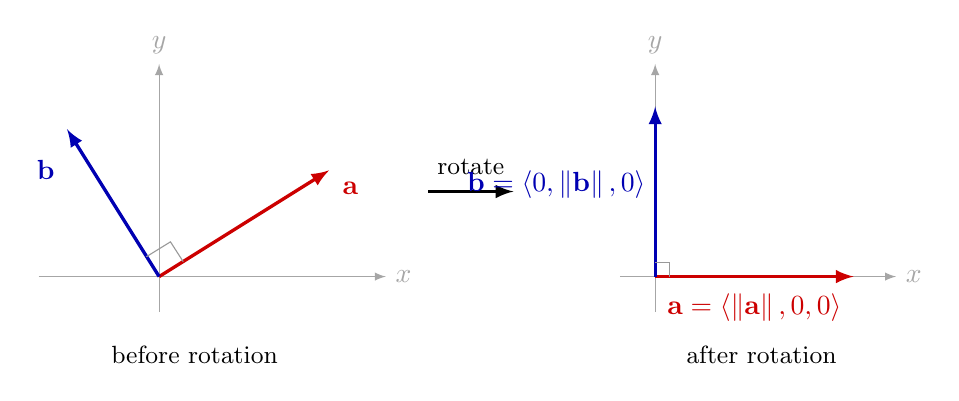
\begin{tikzpicture}[>=latex, scale=0.9]
  % Before
  \begin{scope}
    \draw[->, thin, gray!70] (-1.7, 0) -- (3.2, 0) node[right] {$x$};
    \draw[->, thin, gray!70] (0, -0.5) -- (0, 3) node[above] {$y$};
    \draw[->, very thick, red!80!black] (0,0) -- (2.4, 1.5);
    \node[red!80!black] at (2.7, 1.25) {$\vect{a}$};
    \draw[->, very thick, blue!70!black] (0,0) -- (-1.3, 2.08);
    \node[blue!70!black] at (-1.6, 1.5) {$\vect{b}$};
    % right angle marker at origin between a and b
    \draw[gray!80] (0.34, 0.21) -- ({0.34 - 0.18}, {0.21 + 0.28}) -- ({-0.18}, 0.28);
    \node at (0.5, -1.1) {\small before rotation};
  \end{scope}
  % arrow
  \draw[->, very thick] (3.8, 1.2) -- (5, 1.2);
  \node at (4.4, 1.55) {\small rotate};
  % After
  \begin{scope}[xshift=7cm]
    \draw[->, thin, gray!70] (-0.5, 0) -- (3.4, 0) node[right] {$x$};
    \draw[->, thin, gray!70] (0, -0.5) -- (0, 3) node[above] {$y$};
    \draw[->, very thick, red!80!black] (0,0) -- (2.8, 0);
    \node[red!80!black, below] at (1.4, -0.1) {$\vect{a} = \langle \norm{\vect{a}},0,0\rangle$};
    \draw[->, very thick, blue!70!black] (0,0) -- (0, 2.4);
    \node[blue!70!black, left] at (0, 1.3) {$\vect{b} = \langle 0, \norm{\vect{b}}, 0\rangle$};
    % right angle at origin
    \draw[gray!80] (0.2, 0) -- (0.2, 0.2) -- (0, 0.2);
    \node at (1.5, -1.1) {\small after rotation};
  \end{scope}
\end{tikzpicture}
\end{center}

In these new coordinates the vectors have the simplest possible components,
\[
  \vect{a} = \langle \norm{\vect{a}},\,0,\,0\rangle, \qquad \vect{b} = \langle 0,\,\norm{\vect{b}},\,0\rangle,
\]
so the component formula gives
\[
  \vect{a}\cdot\vect{b} \;=\; \norm{\vect{a}}\cdot 0 \;+\; 0\cdot\norm{\vect{b}} \;+\; 0\cdot 0 \;=\; 0.
\]

By coordinate invariance, the same number $0$ is what the component formula gives in the \emph{original}, pre-rotation axes — even though the original components $a_x, a_y, a_z$ and $b_x, b_y, b_z$ were not zero. Hence $\vect{a}\cdot\vect{b} = 0$ for any perpendicular $\vect{a}$ and $\vect{b}$, no matter which coordinate system we computed it in.

\subsection*{A concrete example}

Take $\ihat = \langle 1,0,0\rangle$ and $\jhat = \langle 0,1,0\rangle$. These are perpendicular by construction, and both arguments agree:
\[
  \ihat\cdot\jhat \;=\; \norm{\ihat}\,\norm{\jhat}\,\cos 90^\circ \;=\; 1\cdot 1\cdot 0 \;=\; 0,
\]
\[
  \ihat\cdot\jhat \;=\; (1)(0) + (0)(1) + (0)(0) \;=\; 0. \checkmark
\]

This tiny computation is the seed of the general statement. Every perpendicular pair of vectors \emph{is} just a rotated, rescaled copy of $(\ihat, \jhat)$, and the dot product respects rotations and scalings — so whatever works for $\ihat\cdot\jhat$ works for any perpendicular pair.

\section{Summary}

We have shown three things.

First, the two definitions
\[
  \vect{a}\cdot\vect{b} = \norm{\vect{a}}\norm{\vect{b}}\cos\theta \quad\text{and}\quad \vect{a}\cdot\vect{b} = a_x b_x + a_y b_y + a_z b_z
\]
agree. The first tells you the geometric meaning: it is the scalar projection of one vector onto the other, scaled by the length of the second. The second is what you get when you expand the first in an orthonormal basis and use the relations $\ihat\cdot\ihat=1$, $\ihat\cdot\jhat=0$, and so on. Every $a_i b_i$ term is a shadow-times-shadow on one coordinate axis; the six cross-terms vanish \emph{because} the axes are perpendicular.

Second, because the geometric formula depends only on lengths and an angle — all coordinate-free quantities — the dot product is invariant under rotations of the coordinate system. The algebraic sum $\sum a_i b_i$ equals the same number in every orthonormal basis, even though the individual components shift around.

Third, perpendicularity detects itself in two equivalent ways: $\cos 90^\circ = 0$ makes the geometric formula vanish, and coordinate invariance lets us rotate any perpendicular pair onto the axes and read the zero directly from the component sum. The example $\ihat\cdot\jhat = 0$ is the archetype; every other perpendicular pair is just a rotated copy of it.

Whenever you see $\sum a_i b_i$ in a calculation — and you will, constantly, in physics and in linear algebra — you are really looking at $\norm{\vect{a}}\norm{\vect{b}}\cos\theta$ in disguise.

\end{document}